\documentclass{article}
\usepackage{graphicx} % Required for inserting images
\usepackage{authblk} % Required for author affiliations
\usepackage{indentfirst} % Indent first paragraph of sections
\usepackage{amssymb} % For mathematical symbols
\usepackage{amsthm} % For theorem environments
\usepackage{amsmath} % For advanced math typesetting
\usepackage{hyperref}
\usepackage{enumitem}
\usepackage{pgfplots} % For plots
\usepackage{tikz} % For drawing shapes
\usepackage{circuitikz}
\pgfplotsset{compat=1.18} % Set compatibility level
\newtheorem{theorem}{Theorem}
\newtheorem{corollary}{Corollary}[theorem]
\newtheorem{lemma}[theorem]{Lemma}
\newtheorem{definition}{Definition}
\newtheorem{problem}{Problem}
\newtheorem{solution}{Solution}
\newtheorem*{example}{Example}
\newtheorem{remark}{Remark}
\newtheorem{proposition}{Proposition}
\reversemarginpar
\hypersetup{
    colorlinks=true,
}
\begin{document}
%------- Title page   -----------
\title{MATH 325: Honours Ordinary Differential Equations}
\author{William Homier}
\affil[1]{McGill University Physics, 3600 Rue University, Montréal, QC H3A 2T8, Canada}
\date{January \(6^{th}\), 2026}
\setcounter{Maxaffil}{0}
\renewcommand\Affilfont{\itshape\small}
\maketitle

%------- Abstract -----------
\noindent\rule{\textwidth}{0.4pt}
\thispagestyle{empty}
\begin{abstract}

\end{abstract}
\noindent\rule{\textwidth}{0.4pt}
\clearpage

%------- Table of Contents -----------
\thispagestyle{empty}
{
  \hypersetup{linkcolor=black}
  \tableofcontents
}
\clearpage

%------- introduction -----------
\setcounter{page}{1}
\section{Introduction}
\section{Prerequisite knowledge}
\section{Basics \& Voltage, Current and Resistance}
\marginpar{January 13, 2026}
\subsection{Signal Types}
\subsubsection{Digital Signal}
\begin{definition}
    A discretely sampled signal with a sequence of quantized values.
\end{definition}
\subsubsection{Analogue}
\begin{definition}
    A continuous signal (e.g., in time) representing (analogous to) some other quantity.
\end{definition}
\begin{example}
    Examples of analogue devices and computers are thermometers, sextants, and tide-predicting machines.
\end{example}
\subsection{Circuits}
\subsubsection{DC}
\begin{definition}
    Direct Current (DC) is a form of current where voltage and current are constant over time, could be found in batteries.
\end{definition}
\begin{definition}
    A DC offset is the addition of a constant DC value to an AC signal.  
    This shifts the entire signal up or down relative to the \(0\,\text{V}\) level, without changing the shape of the AC signal.
\end{definition}

\subsubsection{AC}
\begin{definition}
    Alternating Current (AC) is a form of current that changes over time, often in a sinusoidal manner. AC currents are commonly used in power distribution systems, such as household electrical outlets.
\end{definition}

\subsection{Waves}
\subsubsection{Properties of waves}
To describe waves, considering a sinusoidal wave of the form \(A_psin(2\pi vt)\), we use the following terms
\begin{itemize}
    \item Peak amplitude (\(A_p\)): maximum value of the wave from its equilibrium position .
    \item Peak-to-peak amplitude: total height of the wave from its maximum to its minimum value (i.e., \(2A_p\)).
    \item Frequency (\(v\)): number of cycles per second (Hz).
    \item Time (\(t\)): time variable.
\end{itemize}
To be able to describe AC signals effectively, we take the root mean square (RMS) amplitude \(\frac{A_p}{\sqrt{2}}\) of values such as current and voltage. This is because the mean value of an AC signal is zero, and the RMS is a more meaningful measure of the signal's amplitude as it gives a positive value that is proportional to the energy in the signal.
\[I_{RMS} = \frac{I_p}{\sqrt{2}}\]
\[V_{RMS} = \frac{V_p}{\sqrt{2}}\]

\subsubsection{Waveforms}
\begin{definition}
A waveform is a graphical representation of how a signal varies over time, and can take various forms such as a sine wave, square wave, triangle wave, or sawtooth wave.
\end{definition} 

\paragraph{Direct current (DC).}
A direct current is constant in time, so its graph is a horizontal line.
\begin{center}
\begin{tikzpicture}[scale=1.1]
    % Axes
    \draw[->] (0,0) -- (5,0) node[right] {$t$};
    \draw[->] (0,0) -- (0,5) node[above] {$I(t)$};

    % DC graph
    \draw (0,3) -- (5,3);
\end{tikzpicture}
\end{center}

\paragraph{Alternating current (AC).}
An alternating current varies periodically in time and typically oscillates about zero.
\begin{center}
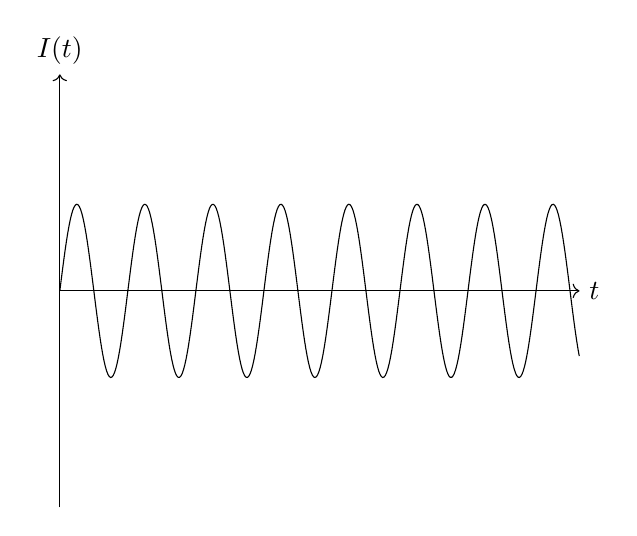
\begin{tikzpicture}[scale=1.1]
    % Axes
    \draw[->] (0,2.5) -- (6,2.5) node[right] {$t$};
    \draw[->] (0,0) -- (0,5) node[above] {$I(t)$};

    % AC graph
    \draw[domain=0:6, samples=400] plot (\x,{sin(8*\x r)+2.5});
\end{tikzpicture}
\end{center}

\paragraph{Pulsating current (DC + AC).}
A pulsating current is an alternating current superimposed on a non-zero DC level. This is just a matter of adding a constant DC level to an AC signal so that the signal is either shifted up or down with respect to the zero current level.
\begin{figure}[h]
    \centering
    \includegraphics[width=0.5\textwidth]{../Images/Pulsating-direct-current-diagram.svg}
    \caption{Pulsating direct current diagram}
    \label{fig:pulsating-direct-current-diagram}
\end{figure}

\subsection{Linear Systems}
\begin{definition}
    Linear systems are systems whose output can be expressed as a linear combination of the input signal(s). The principles of superposition and scaling define the properties of linear systems, where superposition means that the output of a linear system due to the addition of two input signals is the same as the sum of the outputs due to each of the input signals, and scaling means that the output of a linear system due to a scaled input signal is the same as the scaled output due to the original input signal.
\end{definition}
\begin{example}
    Consider two inputs $x_1(t)$ and $x_2(t)$ to a linear system producing outputs $y_1(t) = H[x_1(t)]$ and $y_2(t) = H[x_2(t)]$, where $H$ is some transformation function.

    A linear transformation must satisfy:
    \[y_{total} = \alpha y_1(t) + \beta y_1(t) = H[\alpha x_1(t) + \beta x_2(t)],\]
    where \(\alpha\) and \(\beta\) are constants.
\end{example}
\begin{example}[Superposition]
    \[H[x_1(t) + x_2(t)] = H[x_1(t)] + H[x_2(t)]\]
\end{example}
\begin{example}[Scaling]
    \[H[\alpha x(t)] = \alpha H[x(t)]\]
\end{example}
\subsection{Electric Charge}
\begin{definition}
    Charge is a fundamental physical property that comes in two types: positive (+) and negative (-) (which cancel). Positive and negative charge are usually present in matter in exactly equal proportion (so matter is typically electrically neutral). Charge is conserved—can neither be created nor destroyed and is quantized in units of electronic charge $e = 1.6 \times 10^{-19} \text{C}$.
\end{definition}
\subsection{Current flow}
\begin{definition}[Electric Current]
    Charge per unit time passing a given point in a circuit.
\end{definition}
\begin{definition}[Current Flow]
    The flow of electrons through a wire driven by an electric field potential energy difference. Defined as the rate of charge past a point in a circuit:
    \[I[ampere] = \frac{Q[coulomb]}{time[seconds]}\]
\end{definition}
\begin{definition}[Voltage]
    The electric potential energy divided by the charge. It is the energy per unit charge.
    \[V[volt] = \frac{\Delta E_{Electric}[joule]}{Q[coulomb]}\]
\end{definition}
\begin{definition}[Electron-volt]
    The energy gained or lost by an electron when it moves through an electric potential difference of one volt, which is a unit of energy equal to the work done on an electron in accelerating it through a potential difference of 1V, equal to $1.6 \times 10^{-19}$ Joule.
\end{definition}
An electron between two charged plates has an electric potential energy given by
\[\Delta E_{Electric} = q\Delta V\]
which is converted into kinetic energy (KE) when it is ejected from between the plates.

When discussing current in a circuit, we follow the
convention that it refers to the direction of the flow of positive charges.

Batteries store chemical energy potential. The cathode is
surrounded by positively charged ions, and the anode by
negatively charged ions. Electrons travel through a circuit
from the anode to the cathode, releasing the stored
chemical energy.

\subsection{Electric Field \& Potential}
Charge emits an electric field that exerts a force on other charges. The electric field \(\vec{E}\) at a point in space is defined as the force \(\vec{F}\) experienced by a small positive test charge \(q\) placed at that point, divided by the magnitude of the test charge:
\[\vec{E} = \frac{\vec{F}}{q}\]

It takes work to move a charge against an electric field. The electric potential \(V\) at a point in space is defined as the work needed to move a positive test charge \(W\) per unit charge:
\[V = \frac{W}{q} = -\int_{\vec{r_1}}^{\vec{r_2}}\vec{E}\cdot d\vec{l}\]
If the electric field is uniform, this simplifies to
\[V = -\vec{E}\cdot \vec{d}\]
where \(\vec{d}\) is the displacement vector from point \(\vec{r_1}\) to point \(\vec{r_2}\).

\subsection{Potential \& Ground}
\begin{definition}[Circuit ground]
    The reference point in a circuit at which the electric potential is defined to be zero. All voltages \(V\) in a circuit are measured relative to this point. The symbol for circuit ground is \begin{circuitikz}\draw (0,0) node[ground]{};\end{circuitikz}, and the symbol for chassis ground is \begin{circuitikz}\draw (2,0) node[sground]{};\end{circuitikz}.
\end{definition}
\begin{definition}[Earth ground]
    The earth ground is a possible reference point, which is literally a metal stake or pipe tapped into the soil.
\end{definition}
\subsection{Electromotive Force}
\marginpar{January 15, 2026}
\begin{definition}
    Electromotive Force (EMF)\footnote{EMF is the total energy per unit charge from a source, while voltage is the potential difference measured across points in a circuit, typically less than the EMF due to internal resistance in real sources.} is the energy provided per unit charge by a source such as a battery or generator. It is the work done to move a charge through the source, measured in volts (V).
\end{definition}

To better understand the concept of EMF, consider the following analogy: EMF is like a voltage credit that is then all spent by dropping it over the elements of the circuit. Think of your checking account with two columns: credit (money in) and debit (money spent). EMF is like the "credit" that is then all "spent" by dropping it over the elements of the circuit.
\subsubsection{Faraday's Law}
\begin{theorem}
    Faraday's Law states that a changing magnetic flux through a closed loop induces an electromotive force (EMF) in the loop. Mathematically, it is expressed as:
    \[\mathcal{E}_{EMF} = -\frac{d\Phi_B}{dt}\]
    where \(\mathcal{E}_{EMF}\) is the induced EMF, and \(\Phi_B\) is the magnetic flux through a wire loop, defined as:
    \[\Phi_B = \int B \cdot da\]
\end{theorem}

\subsection{Ohm's Law}
\begin{definition}
    Ohm's Law states that the current \(I\) flowing through a conductor is directly proportional to the voltage \(V\) across it and inversely proportional to its resistance \(R\). Mathematically, it is expressed as:
    \[I = \frac{V}{R}\]
\end{definition}
Microscopically, Ohm's Law can be understood in terms of the motion of electrons in a conductor. When a voltage is applied across a conductor, it creates an electric field that exerts a force on the free electrons, causing them to move and create an electric current. The resistance of the conductor arises from collisions between the electrons and the atoms in the material, which impede their motion. The greater the resistance, the more collisions occur, resulting in a lower current for a given voltage.
The current density \(J\) is given by Ohm's Law, which states that the current density is proportional to the electric field strength \(E\):
\[J = \sigma E\]
Conversely, the electric field strength is given by the current density and the resistivity of the material:
\[E = J\rho_r\]
The current \(I\) is given by the current density and the cross-sectional area of the material:
\[I = AJ = A\sigma E\]
The electric field strength can also be expressed in terms of the potential difference \(\Delta V\) across the material and its length \(l\):
\[E = \Delta V/l\]
Substituting this into the expression for the current, we obtain:
\[I = \frac{A\sigma \Delta V}{l} = \frac{A\Delta V}{\rho_r l}\]
The potential difference across the material is also given by the resistance \(R\) and the current \(I\) as stated in Ohm's Law:
\[\Delta V = IR\]
Finally, the resistance can be expressed in terms of the resistivity of the material, the length of the material, and its cross-sectional area:
\[R = \frac{\rho_r l}{A}\]

Ohm's Law can be represented graphically using the Ohm's Law Wheel, which illustrates the relationships between current, voltage, resistance, and conductance. The wheel is a useful tool for quickly finding the value of one electrical property given the values of the other three.
\begin{figure}[h]
    \begin{center}
        \includegraphics[width=0.5\textwidth]{../Images/Ohms-Law-Formula-Wheel.png}
        \caption{Ohm's Law Wheel and Current Density}
    \end{center}
\end{figure}

\subsection{Resistors}
\begin{definition}
    A resistor is a device that opposes the flow of current through it, resulting in a voltage drop across it. Resistors are characterized by their resistance value \(R\), measured in ohms (\(\Omega\)), which quantifies the amount of opposition they provide to the flow of current. According to Ohm's Law, the voltage drop \(V\) across a resistor is directly proportional to the current \(I\) flowing through it:
    \[V = IR\]
\end{definition}
When resistors are connected in series, their resistances add together to form a total resistance $R_{tot} = R_1 + R_2 + \cdots + R_n$. In contrast, when resistors are connected in parallel, their resistances add inversely to form a total resistance $\frac{1}{R_{tot}} = \frac{1}{R_1} + \frac{1}{R_2} + \cdots + \frac{1}{R_n}$.
\begin{figure}
    \begin{center}
        \includegraphics[width=0.5\textwidth]{../Images/Parallel_resistors.png}
        \caption{In all of these examples, the components are wired in parallel.}
    \end{center}
\end{figure}
\subsubsection{Temperature Dependence}
The temperature dependence of the resistance of many metals can be modelled by the following equation:
\[R_T = R_0[1 + \alpha (T - T_0)]\]
where \(R_0\) is the resistance value at reference temperature \(T_0\), and \(\alpha\) is the linear temperature coefficient. This equation shows that the resistance of a metal increases linearly with temperature, which is a common phenomenon observed in many metals.
\subsubsection{Power Dissipation}
When current flows through a resistor, electrical energy is converted into heat energy due to the resistance of the material. The power \(P\) dissipated by a resistor can be calculated using the formula:
\[P = \Delta V \cdot I\]
Using Ohm's Law, we can express the power dissipated in terms of the resistance \(R\) and either the voltage drop \(\Delta V\) or the current \(I\):
\[P = I^2 R = \frac{(\Delta V)^2}{R}\]
\subsection{Batteries}
\marginpar{January 20, 2026}
\begin{definition}[Ideal Battery]
    An ideal battery is a theoretical concept that represents a perfect voltage source with no internal resistance. It maintains a constant voltage output regardless of the current drawn from it, meaning that it can supply any amount of current without any voltage drop or loss of energy.
\end{definition}
\begin{definition}[Real Battery]
    A real battery, on the other hand, has internal resistance that causes a voltage drop when current is drawn from it. This means that the voltage output of a real battery decreases as the current increases, leading to a loss of energy in the form of heat due to the internal resistance.
\end{definition}
The circuit containing a real battery can be modeled as an ideal voltage source \(V_0\) or \(V_{ideal}\) in series with an internal resistance \(r\). The terminal voltage \(V_{terminal}\) of the battery when a current \(I\) is drawn from it can be expressed as:
\[V_{terminal} = V_{0} - Ir\]
However, if the circuit contained a resistor \(R\) connected to the battery, the current \(I\) flowing through the circuit can be calculated using Ohm's Law:
\[V_0 = Ir + IR\]

\subsection{Static Circuits and Electronics}
Consider the variation of electric potential along a conducting wire. 
If the wire has a small but non-negligible resistance that is uniformly distributed, the potential decreases approximately linearly with distance along the wire, since the voltage drop is proportional to length.
\begin{center}
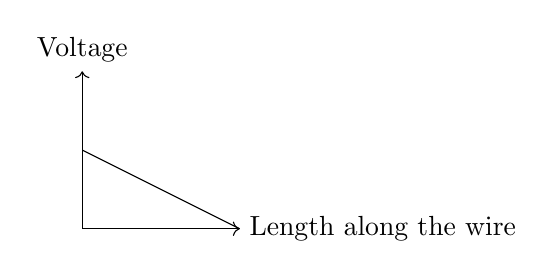
\begin{tikzpicture}
    \draw[->] (0,0) -- (2,0) node[right] {Length along the wire};
    \draw[->] (0,0) -- (0,2) node[above] {Voltage};

    \draw[domain=0:2] plot (\x, {1-0.5*\x});
\end{tikzpicture}
\end{center}
In contrast, if a discrete resistor with resistance much larger than that of the wire is introduced, nearly all of the voltage drop occurs across the resistor. The potential along the wire remains approximately constant, with a sharp decrease only at the location of the resistor.
\begin{center}
\begin{tikzpicture}
    \draw[->] (0,0) -- (2,0) node[right] {Length along the wire};
    \draw[->] (0,0) -- (0,2) node[above] {Voltage};

    \draw (0,1) -- (1.6,1);
    \draw (1.6,0.1) -- (2,0.1);
    \draw (1.6,1) -- (1.6,0.1);
\end{tikzpicture}
\end{center}



\section{Circuit Theory Beyond Electronic}
\section{Capacitors \& Inductors}
\section{RC and LR Circuits with AC Driving}
\section{Impedance}
\section{RLC Circuits}
\subsection{Transient Response}
\subsection{Driven RLC Circuits}
\subsection{Power Input to RLC and Circuit Network}
\section{Circuit Networks}
\section{Fourier Series}
\section{Fourier Transforms}


\section{Appendix}

\section{Useful Links}

\end{document}